\section{Introduction}

\paragraph{Background} \cite{SoC-market}

The chip industry's focus is shifting from personal computing to 
a plethora of small, intelligent devices. The internet of things, intelligent cars,
smart phones and drones are only examples of the devices that draw the chip industry's 
attention more and more. 
Some common properties of such devices that force chip producers to shift their attention 
from transistor level to core level are:

\begin{enumerate}
\item The need for integration of multiple powerful functionalities into a small device
\item The need for power efficiency, because of power dissipation in nanoscale VLSI circuits. 
\item The need for cost reduction due the growth of chip producing competitors in these markets.
\item The need for improvement of time to market using combined intellectual propertie in a product.
\end{enumerate}

These issues illustrate the importance of further integration and the
related technologies that makes this possible. The next section introduces these technologies.

\paragraph{SoC}

An integrated circuit that covers multiple cores or intellectual properties
blocks (IP's) which are linked to an internal bus system is called a system on
chip or SoC. IP's of several companies are integrated into a single chip. So the
SoC producer can focus on its core business instead of building all the
functionality by themselves and reduce time to market. But the more IP's attached
to a traditional bus system the wiring delay increases exponential and longer
wiring reduces the bus its bandwidth.\cite{SoC}

\paragraph{NoC}

The use of network communication inside a chip instead of a traditional bus
system is inevitable. One of the reasons is to cope with the increasing number
of cores into a single chip. It is also less complex to integrate IP's from
different companies. A so called network on chip or NoC has much less wiring
\cite{NoC-busses} and can handle more IP's without losing performance. For the
related business it has the same advantage as it does for network communication
in general:

\textit{``Replacement of SoC busses by NoC's will follow the same path of data
communications when the economics prove that the NoC either reduces SoC
manufacturing cost, SoC time to market, SoC time to volume, and SoC design risk
or increases SoC performance.''} \cite{NoC-busses} 

The success of the NoC design depends on the research of the interfaces between
processing elements of NoC and interconnection fabric.

\paragraph{xMAS}

If a NoC does not meet its specification or isn't reliable e.g. because of
deadlock situations in the network, the cost of production loss is much higher
than the costs spent for the extra design or verification effort. In worst case
a company can lose its market share and reputational damage. It is very
important to detect flaws in an early stage of NoC production process, therefore
researchers have developed a high level modeling language for communication
fabrics called xMAS or executable Micro Architectural Specifications. This high
level approach makes modeling less complex and gives researchers a way to gain
knowledge of how these fabrics behave under certain conditions so they can prove
the absence or presence of specific properties long before it's built on
silicon.

xMAS consists of only eight primitive components. Each component has one or more
ports. To create a valid model all ports must be connected by channels. Some
components have specific properties to set. These properties are used by the
verification tools. E.g. the queue has a size property. Once a model has been
created and all components are set up it can be verified to detect deadlock
situations or other flaws.

\begin{figure}[here]
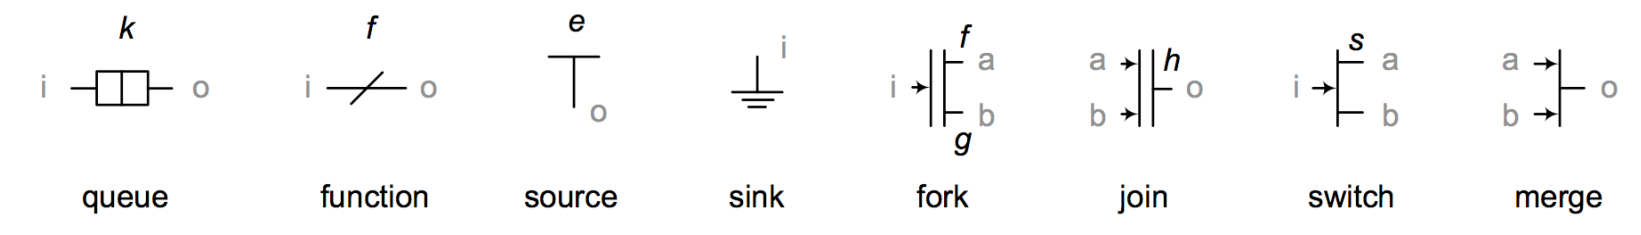
\includegraphics[width=1.0\textwidth]{xmas-language}
\caption{Eight primitives of the xMAS language \cite{6225465}. Italicized letters indicate
parameters. Gray letters indicate ports.}
\label{fig:xmas-language}
\end{figure}

\paragraph{Design and verification tools}

To make use of the xMAS language and verification tools, computer scientists
have developed an application called WickedXMAS \cite{WickedXmas}.
With this application it is possible to draw a model and export it so it can be
verified. The verification tool reads the model and processes one or more
algorithms e.g. to detect network deadlocks or model syntax faults.

Although the WickedXMAS designer tool is still useful and unique in its kind
there are some major shortcomings and had to be redesigned because:
\begin{enumerate}
\item It was written in csharp which makes it only available for researchers
working on a Windows platform.
\item Verification tools are not integrated which
makes it complicated to use.
\item The model must be exported before it can be
used by the verification tools.
\item It is difficult to maintain, verification tools are written in c++ while
designer is written in csharp and xaml
\item The tool aborts in several situations.
\item Lack of composite management.
\item Recursive composite feature not working.
\end{enumerate}

Therefore our team was asked to design and build a new tool. Our goal was to
create a maintainable, platform independent, xMAS modeling tool that integrates
the verification tools.
By integrating formal verification into a new designer-friendly tool, a designer
can easily verify a design.

The project is split into a designer that we call
``xmd'' or xMAS Model Designer and the verification process called ``xmv'' or
xMAS Model Verification. The project is based on Qt's latest technology where we
have written the GUI in QML (JavaScript) and the logic in c++.

Instead of implementing specific verification tools we have put our effort into
implementing a generic plug-in interface. Via this interface, verification tools
can be easily plugged in and controlled. This interface can also send the
verification results to the console.
\begin{wrapfigure}{r}{0.55\textwidth}
  \vspace{-20pt}
  \begin{center}
    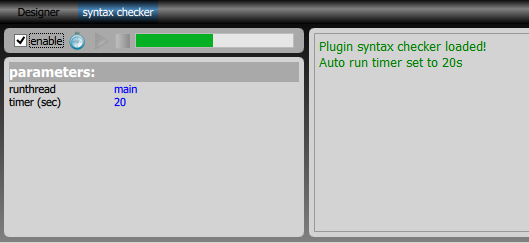
\includegraphics[width=0.50\textwidth]{console}
  \end{center}
  \vspace{-20pt}
  \caption{xmd syntax checker plug-in console}
  \label{fig:console}
  \vspace{-10pt}
\end{wrapfigure}
A scientist can easily implement a new verification algorithm if it has the
plug-in interface. We have provided the syntax checker of such a plug-in interface
that can be used as an example for other verification tools. Each plug-in
automatically gets its own console output and control with setup fields.
Starting a verification process is simply done by clicking the start button, no
conversion or exports are necessary anymore.


In the new designer ``xmd'' all actions on the canvas are now directly reflected
into the model network and can be verified immediately. Another improvement of
the designer is the management of composite components, which are subnetworks
that can be reused and make it possible to quickly build large models in an easy
way.
\begin{wrapfigure}{r}{0.55\textwidth}
  \vspace{-20pt}
  \begin{center}
    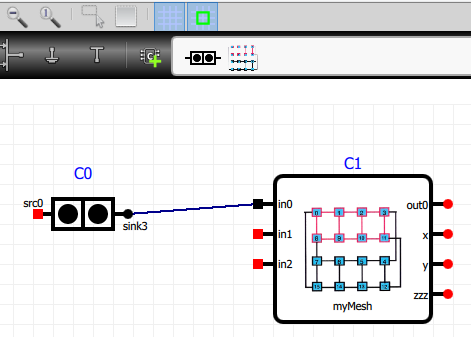
\includegraphics[width=0.50\textwidth]{composite-use}
  \end{center}
  \vspace{-20pt}
  \caption{xmd composite library and canvas use}
\label{fig:composite-use}
  \vspace{-10pt}
\end{wrapfigure}
A model can be setup with composite properties so it can be used just
like a primitive. A designer can do this by adding them to a model its composite
library and drag those into the canvas. The way that xmd implements composites
gives scientists the opportunity to extend these with a parametric expression.
With a parametric expression it is possible to call a composite in a recursive
way and avoid drawing large networks of already valid subnets.

\newpage